\documentclass[../main.tex]{subfiles}

\begin{document}

\subsection{Szablony HTML}
Frontend aplikacji został zrealizowany przy pomocy szablonów \texttt{HTML} wspieranych przez framework \texttt{Django}. Aplikacja zawiera następujące szablony HTML:

\begin{itemize}
	\item \texttt{base.html}
	      \begin{itemize}
		      \item Bazowy szablon dla wszystkich stron w aplikacji.
		      \item Zawiera nagłówek, stopkę, podstawowe style oraz logikę nawigacji.
		      \item Nagłówek zawiera linki do różnych stron: Strona Główna, Filmy, Szczegóły filmu, O nas,  użytkownicy
		      \item Renderuje blok `content`, który jest nadpisywany w zależności od podstrony.
	      \end{itemize}
	\item \texttt{movies.html}
	      \begin{itemize}
		      \item Wyświetla listę filmów oraz szczegóły każdego z nich.
		      \item Używa pętli do iterowania przez filmy i wyświetlania ich szczegółów takich jak tytuł, rok produkcji,  ocena, liczba głosów, gatunki, reżyserzy oraz obsada.
		      \item Filmy są prezentowane w formie kart z obrazkami plakatów i krótkimi opisami.
		      \item Każdy film jest linkiem do szczegółów danego filmu.
	      \end{itemize}
	\item \texttt{movie\_details.html}
	      \begin{itemize}
		      \item Wyświetla szczegóły pojedynczego filmu.
		      \item Zawiera szczegółowe informacje o filmie: tytuł, rok produkcji, ocena, gatunki, reżyserzy, obsada oraz zdjęcie plakatu.
	      \end{itemize}
	\item \texttt{add\_comment.html}
	      \begin{itemize}
		      \item Formularz do dodawania komentarzy do filmu.
		      \item Użytkownik może wprowadzić tekst komentarza i wysłać formularz metodą \texttt{POST}.
		      \item Formularz zawiera zabezpieczenie \texttt{CSRF} (Cross-Site Request Forgery).
	      \end{itemize}
	\item \texttt{add\_review.html}
	      \begin{itemize}
		      \item Formularz do dodawania recenzji filmu.
		      \item Użytkownik może ocenić film w skali od 1 do 5 oraz dodać swoją recenzję tekstową.
	      \end{itemize}
	\item \texttt{about.html}
	      \begin{itemize}
		      \item Strona z informacjami o aplikacji.
	      \end{itemize}
	\item \texttt{login.html} oraz {register.html}
	      \begin{itemize}
		      \item Formularze logowania i rejestracji nowych użytkowników.
		      \item Logowanie wymaga podania loginu i hasła, natomiast rejestracja obejmuje dodatkowe pola, takie jak imię, nazwisko i email.
	      \end{itemize}
	\item \texttt{user\_details.html}
	      \begin{itemize}
		      \item Wyświetla szczegóły dotyczące użytkownika.
		      \item Zawiera informacje o użytkowniku, jego recenzjach oraz ulubionych filmach.
	      \end{itemize}
\end{itemize}

\subsection{CSS}

% Fake nagłówek
\newcommand{\fakesection}[1]{
	\FloatBarrier % nie pozwól rysunkom "uciekać" do innych fakesekcji
	\vspace{\baselineskip} 
	\noindent \textbf{\large #1}
}

Aplikacja używa pliku CSS do definiowania wyglądu i układu elementów na stronach. Stylizacja opiera się na responsywnym projekcie z ciemnym motywem. W pliku CSS zdefiniowane są m.in. style dla nagłówków, przycisków, kart filmów, formularzy oraz elementów interaktywnych.

\fakesection{Nagłówek i Nawigacja}

Nagłówek aplikacji zawierający nawigację, ma ciemne tło oraz jasny tekst. Linki do poszczególnych stron zmieniają kolor po najechaniu, co daje użytkownikowi jasną wskazówkę interaktywności (rys. \ref{fig:frontend:css_navbar}).

\begin{figure}[htb]
	\centering
	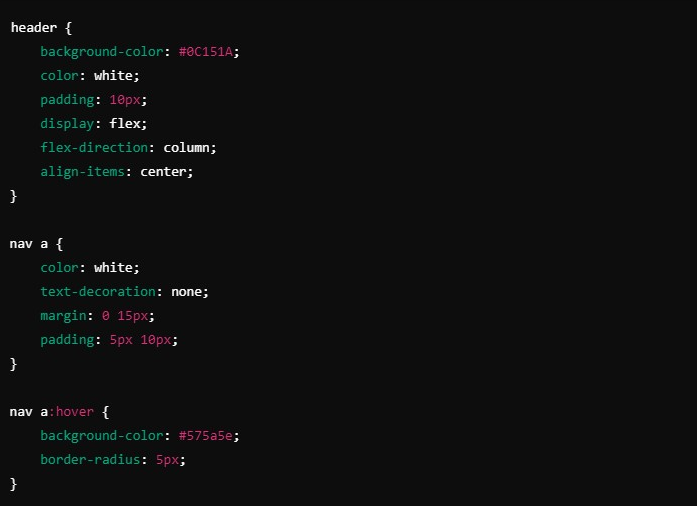
\includegraphics[width=.75\textwidth]{frontend/naglowek_i_nawigacja.png}
	\caption{Styl nagłówków i nawigacji}
	\label{fig:frontend:css_navbar}
\end{figure}

\fakesection{Przyciski}

Przyciski, takie jak te używane do logowania, wylogowania czy przesyłania formularzy, mają zaokrąglone krawędzie i są stylizowane w ciemnych odcieniach. Przycisk zmienia kolor na jaśniejszy po najechaniu kursorem (rys. \ref{fig:frontend:css_buttons}).

\begin{figure}[htb]
	\centering
	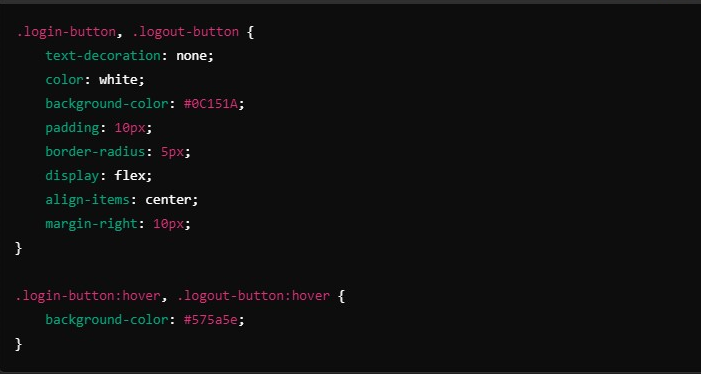
\includegraphics[width=.75\textwidth]{frontend/przyciski.png}
	\caption{Styl przycisków}
	\label{fig:frontend:css_buttons}
\end{figure}

\fakesection{Siatka Filmów i Karty Filmów}

Karty filmów są centralnym elementem aplikacji. Każdy film jest wyświetlany w formie karty z obrazkiem plakatu, tytułem, oceną i innymi szczegółami. Karty są stylizowane tak, aby były wizualnie atrakcyjne, a jednocześnie dobrze zorganizowane i czytelne (rys. \ref{fig:frontend:css_filmy}).
Główne cechy:
\begin{itemize}
	\item Elastyczna siatka (grid)
	\item Cienie i zaokrąglenia
\end{itemize}

\begin{figure}[htb]
	\centering
	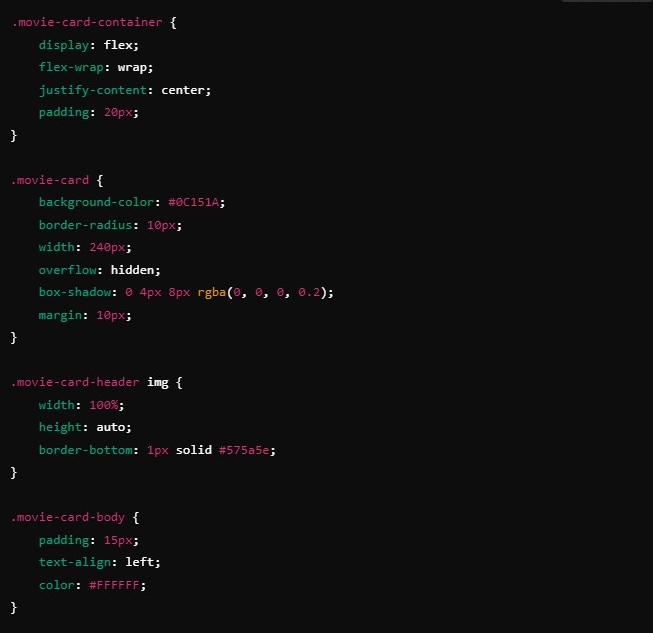
\includegraphics[width=.75\textwidth]{frontend/filmy.png}
	\caption{Styl siatki filmów}
	\label{fig:frontend:css_filmy}
\end{figure}

\fakesection{Sekcja Recenzji}

Recenzje użytkowników są wyświetlane w formie kart, podobnie jak filmy. Zawierają one dane o autorze recenzji, ocenę oraz tekst recenzji. Style kart mają dodatkowe elementy, takie jak gwiazdki oceny (rys. \ref{fig:frontend:css_recenzje}).

\begin{figure}[htb]
	\centering
	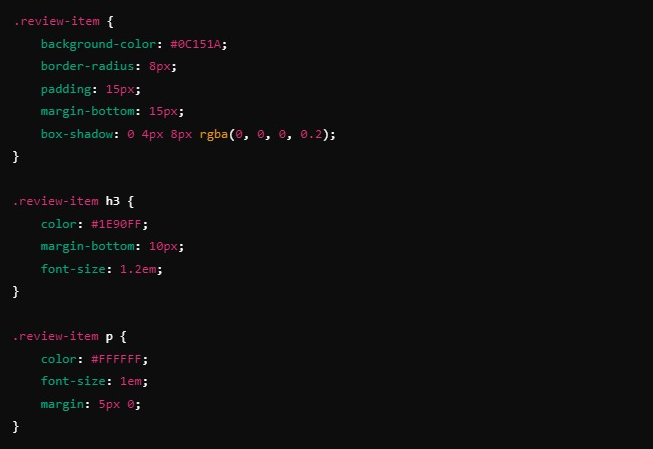
\includegraphics[width=.75\textwidth]{frontend/recenzje.png}
	\caption{Styl siatki recenzji}
	\label{fig:frontend:css_recenzje}
\end{figure}

\fakesection{Formularze}

Formularze takie jak te do dodawania recenzji, komentarzy, logowania oraz rejestracji, są stylizowane w sposób zapewniający intuicyjne korzystanie (rys. \ref{fig:frontend:css_form}).

\begin{figure}[htb]
	\centering
	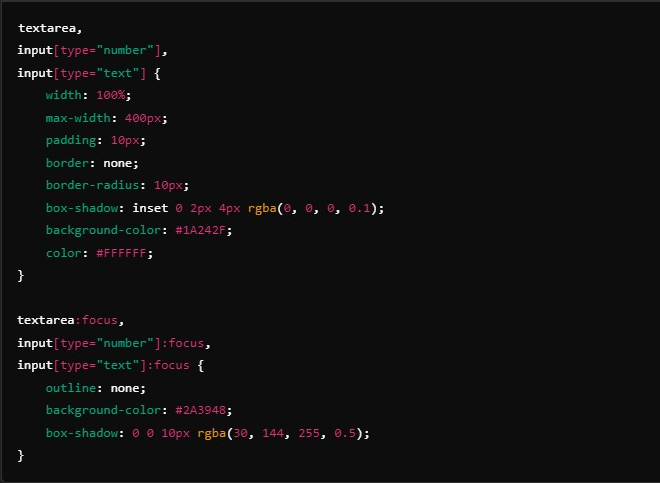
\includegraphics[width=.75\textwidth]{frontend/formularze.png}
	\caption{Styl formularzy}
	\label{fig:frontend:css_form}
\end{figure}

\end{document}